\chapter{Tecnologías utilizadas}\label{chapter:presentacion_del_problema}

 PODRIA IR ACA LA PRESENTACION DEL PROBLEMA
 
 OBJETIVOS
 
\section{ Herramientas de software}
En esta sección se describen las herramientas de software utilizadas para la programación del proyecto.

Pypose: Software especializado en el control de los servomotores Dynamixel Ax-12. Una de las más importantes características es que, luego de haber fijado a mano las posiciones de los motores, permite la lectura simultánea de esas posiciones para captar la pose del robot. Con esta herramienta es posible formar una secuencia de poses que generen un movimiento, por ejemplo, caminar. \cite{pypose}

ROS: ROS (Robot Operating System) es un framework que proporciona bibliotecas y herramientas para ayudar a los desarrolladores de software a crear aplicaciones robóticas. Proporciona abstracción de hardware, controladores de dispositivos, bibliotecas, visualizadores, paso de mensajes, gestión de paquetes y más. ROS se encuentra bajo licencia de código abierto, la licencia BSD.

OpenCv (Open Source Computer Vision Library): Es una librería de visión de computadoras y aprendizaje de maquinas de código abierto. Ha sido diseñada para acelerar el uso de la percepción de maquinas y para proveer una estructura común en las aplicaciones de visión de computadoras. Registrada bajo la licencia BSD, de código abierto. \cite{opencv}

IDE Arduino: Es un entorno de desarrollo para escribir y cargar código en la tarjeta Arduino. Otras tarjetas con microcontroladores AVR también son compatibles, como la Arbotix. El lenguaje de programación del IDE de Arduino es una implementación de Wiring el cual esta basado en Processing.  \cite{arduino}


\section{Componentes de hardware}
En esta sección se describen los principales componentes utilizados para armar la estructura del robot.
\begin{itemize}
\item Bioloid Premium kit: Es un kit de robótica con piezas modulares que permite armar diferentes tipos de robot pero principalmente humanoides. El fabricante, ROBOTIS, incluye un manual con varios modelos de robots con instrucciones de ensamblaje. Provee una tarjeta controladora, CM-530, a la que se conectan los motores Dynamixel y algunos sensores que se programan a través de la interfaz de ‘RoboPlus’.

\end{itemize}

\begin{figure}[hbtp]
\caption{Bioloid Kit}
\centering
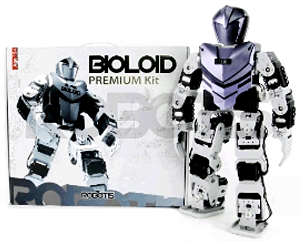
\includegraphics[scale=0.5]{imagenes/product_bioloid17.png}
\end{figure}

\begin{itemize}

\item Motores Dynamixel Ax-12+: Son actuadores inteligentes y modulares que incorporan un reductor de engranajes, un motor DC de presión y un circuito de control con funcionalidad de red, todo en un solo paquete. (R. INC, Dynamixel AX-12, 2006.)
\end{itemize}

\begin{figure}[hbtp]
\caption{Motores Dynamixel conectados en serie}
\centering
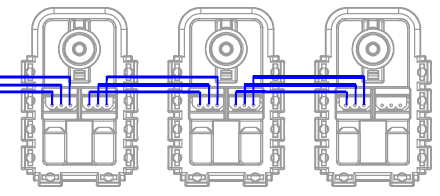
\includegraphics[scale=0.5]{imagenes/AX-12_serie.png}
\end{figure}

\begin{itemize}
\item Gyro: Es un giroscopio de la marca Robotis que mide la velocidad angular, diseñado para mantener el balance del robot y ser usado para otras aplicaciones de movimiento. 

\end{itemize}

Sensor Gyro 
%http://support.robotis.com/en/product/auxdevice/sensor/dxl_gyro.htm
\begin{itemize}
\item Arbotix: El controlador ArbotiX es una solución de control avanzado para manejar servos Dynamixel AX/MX/RX/EX y robots basados en Bioloid. Incorpora un potente microcontrolador AVR, radio inalámbrica XBEE, conductores de motor dual, y cabeceras de estilo servo de 3 pines para E/S digital y analógica.
%http://www.trossenrobotics.com/p/arbotix-robot-controller.aspx 

\end{itemize}
\begin{itemize}
\item FTDI (Future Technology Devices International) : Es una tarjeta controladora que ofrece el servicio de conversión de datos de USB a UART. Permite la comunicación entre diferentes dispositivos. 

Chip FTDI conectado a la tarjeta Arbotix

\end{itemize}


\begin{itemize}
\item Extensor de puertos bioloid : Permite aumentar el número de cadenas de servos conectados a la tarjeta. 

%https://www.bananarobotics.com/shop/Dynamixel-AX-MX-6-Port-Extension-Hub

\end{itemize}


\begin{itemize}
\item Servo motor analogico micro TG9 e: Es un pequeño servomotor cuyo torque alcanza 1.50 kg-cm y una velocidad de 60º por segundo. Permite ser controlado en posición en un rango de 180º. 
Servo motor analogico 
%http://www.hobbyking.com/hobbyking/store/__9549__Turnigy_TG9e_9g_1_5kg_0_10sec_Eco_Micro_Servo.html

\end{itemize}

\begin{itemize}
\item Raspberry Pi: La Raspberry Pi es un ordenador del tamaño de una tarjeta de crédito a la que se puede conectar un televisor y un teclado. Se trata de un pequeño ordenador capaz de ser utilizado en proyectos de electrónica, y para muchas de las tareas que una PC de escritorio hace, como hojas de cálculo, procesadores de texto y juegos. http://www.raspberrypi.org/ 


Tarjeta Raspberry Pi con descripción de los puertos
imagen tomada de: %http://rayhightower.com/blog/2012/12/03/ruby-on-raspberry-pi/

\end{itemize}

\begin{itemize}
\item Camara Raspberry Pi: Es un sensor encargado de captar imagenes y grabar videos de alta definicion. Se conecta a la Raspberry Pi con un cable de cinta plana de 15 cm en el puerto CSI. Tiene 5 megapíxeles de foco fijo que soporta los modos de vídeo de 1080x30, 720x60 y VGA90. Puede ser manejada con las librerías MMAL, V4L u otras librerías de terceros como la de Python. %(http://www.raspberrypi.org/products/camera-module/)

\end{itemize}



Camara Raspberry Pi 
\begin{itemize}
\item Batería de polímero de litio (Lipo): Es la fuente de poder usada para que los motores y componentes electronicos funcionen. La batería usada es de 11.1 voltios y 1 amperio. 
\end{itemize}
\begin{itemize}
\item Circuito con regulador de 5v: Es un circuito diseñado y construido para este proyecto cuya finalidad es regular la entrada de la corriente. Por una de las salidas se expulsa 5v y por la otra se mantiene el mismo voltaje de entrada. 

\end{itemize}



